\documentclass{article}

\usepackage{fancyhdr}
\usepackage{extramarks}
\usepackage{amsmath}
\usepackage{amsthm}
\usepackage{amsfonts}
\usepackage{tikz}
\usepackage{graphicx} %插入图片的宏包
\usepackage{float} %设置图片浮动位置的宏包
% \usepackage{subfigure} %插入多图时用子图显示的宏包
% \usepackage[plain]{algorithm}
% \usepackage{algpseudocode}

% \usetikzlibrary{automata,positioning}

%
% Basic Document Settings
%

\topmargin=-0.45in
\evensidemargin=0in
\oddsidemargin=0in
\textwidth=6.5in
\textheight=9.0in
\headsep=0.25in

\linespread{1.1}

\pagestyle{fancy}
\lhead{\hmwkAuthorName}
\chead{\hmwkClass\ : \hmwkTitle}
\rhead{\firstxmark}
\lfoot{\lastxmark}
\cfoot{\thepage}

\renewcommand\headrulewidth{0.4pt}
\renewcommand\footrulewidth{0.4pt}

\setlength\parindent{0pt}

%
% Create Problem Sections
%

\newcommand{\enterProblemHeader}[1]{
    \nobreak\extramarks{}{Problem \arabic{#1} continued on next page\ldots}\nobreak{}
    \nobreak\extramarks{Problem \arabic{#1} (continued)}{Problem \arabic{#1} continued on next page\ldots}\nobreak{}
}

\newcommand{\exitProblemHeader}[1]{
    \nobreak\extramarks{Problem \arabic{#1} (continued)}{Problem \arabic{#1} continued on next page\ldots}\nobreak{}
    \stepcounter{#1}
    \nobreak\extramarks{Problem \arabic{#1}}{}\nobreak{}
}

\setcounter{secnumdepth}{0}
\newcounter{partCounter}
\newcounter{homeworkProblemCounter}
\setcounter{homeworkProblemCounter}{1}
\nobreak\extramarks{Problem \arabic{homeworkProblemCounter}}{}\nobreak{}

%
% Homework Problem Environment
%
% This environment takes an optional argument. When given, it will adjust the
% problem counter. This is useful for when the problems given for your
% assignment aren't sequential. See the last 3 problems of this template for an
% example.
%
\newenvironment{homeworkProblem}[1][-1]{
    \ifnum#1>0
        \setcounter{homeworkProblemCounter}{#1}
    \fi
    \section{Problem \arabic{homeworkProblemCounter}}
    \setcounter{partCounter}{1}
    \enterProblemHeader{homeworkProblemCounter}
}{
    \exitProblemHeader{homeworkProblemCounter}
}

%
% Homework Details
%   - Title
%   - Due date
%   - Class
%   - Section/Time
%   - Instructor
%   - Author
%

\newcommand{\hmwkTitle}{Quiz\ \#2}
\newcommand{\hmwkDueDate}{Dec 5, 2018}
\newcommand{\hmwkClass}{Complex Networks}
\newcommand{\hmwkClassTime}{Section A}
% \newcommand{\hmwkClassInstructor}{Professor Isaac Newton}
\newcommand{\hmwkAuthorName}{\textbf{RUOPENG XU} }
\newcommand{\hmwkAuthorNum}{\textbf{18M38179} }

%
% Title Page
%

\title{
    \vspace{2in}
    \textmd{\textbf{\hmwkClass:\ \hmwkTitle}}\\
    \normalsize\vspace{0.1in}\small{Due\ on\ \hmwkDueDate\ }\\
    % \vspace{0.1in}\large{\textit{\hmwkClassInstructor\ \hmwkClassTime}}
    \vspace{3in}
}

\author{\hmwkAuthorName\\ \hmwkAuthorNum}
\date{}

\renewcommand{\part}[1]{\textbf{\large Part \Alph{partCounter}}\stepcounter{partCounter}\\}

%
% Various Helper Commands
%

% Useful for algorithms
\newcommand{\alg}[1]{\textsc{\bfseries \footnotesize #1}}

% For derivatives
\newcommand{\deriv}[1]{\frac{\mathrm{d}}{\mathrm{d}x} (#1)}

% For partial derivatives
\newcommand{\pderiv}[2]{\frac{\partial}{\partial #1} (#2)}

% Integral dx
\newcommand{\dx}{\mathrm{d}x}

% Alias for the Solution section header
\newcommand{\solution}{\textbf{\large Solution}}

% Probability commands: Expectation, Variance, Covariance, Bias
\newcommand{\E}{\mathrm{E}}
\newcommand{\Var}{\mathrm{Var}}
\newcommand{\Cov}{\mathrm{Cov}}
\newcommand{\Bias}{\mathrm{Bias}}

\begin{document}

\maketitle

\pagebreak

\begin{homeworkProblem}
    % questions
1. Make a program of counting the number of triangles in “karate club network”. Show the code and its results.

2. Compute the maximum number of triangles in a graph of 9 nodes.

3. Draw a graph of 9 nodes and 12 edges that contains no triangles.

1. Network data is available in the following sites.

http://www‐personal.umich.edu/~mejn/netdata/

http://networkrepository.com/soc‐karate.php

    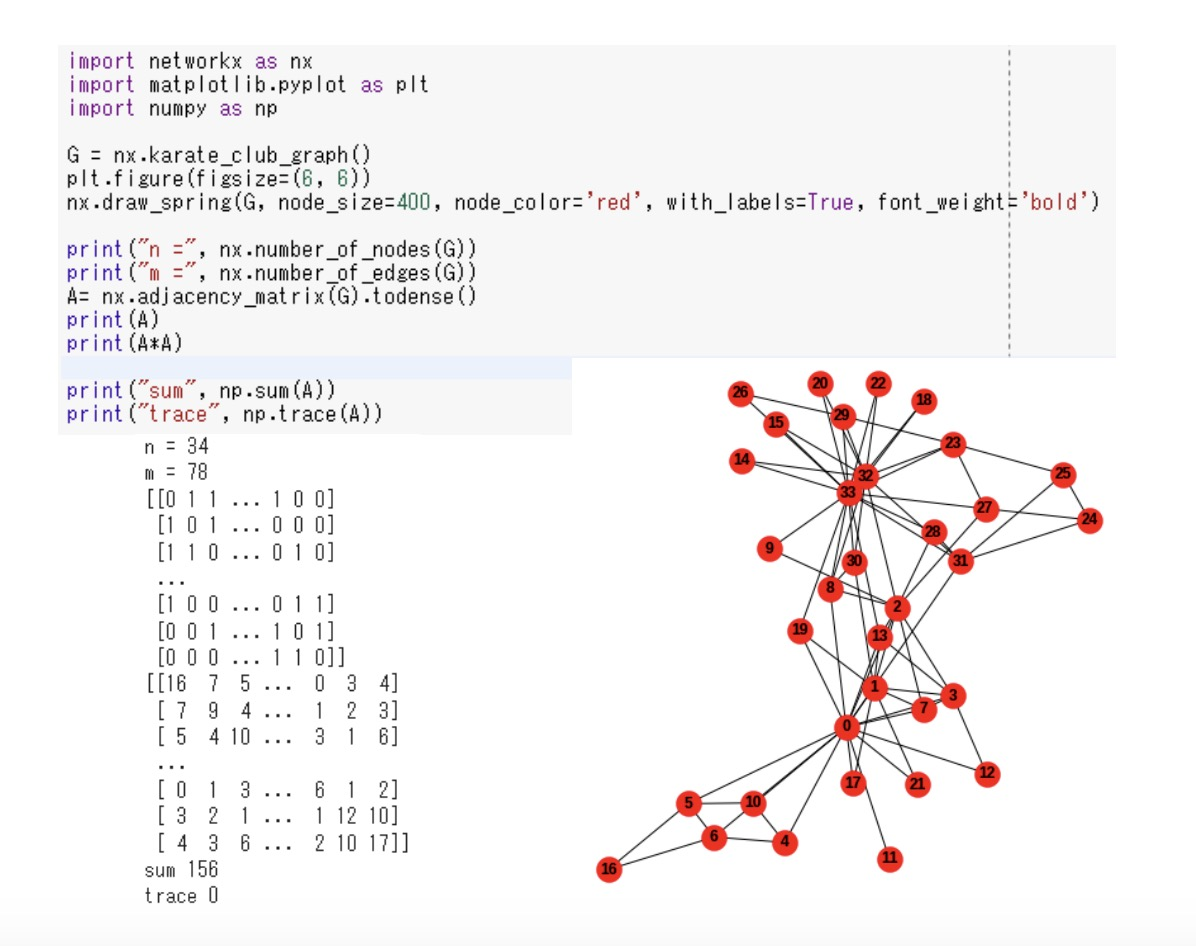
\includegraphics[scale=0.4]{quiz2.jpg}

    \subsection*{Part One}
    figure(b) is a social network and figure(a) is an Internet

    \subsection*{Part Two}
    \subsubsection*{Degree distribution}

    % \textbf{notes:}

    % \emph{-the degree of a node in a network is the number of connections it has to other nodes.}

    % \emph{-the degree distribution is the probability distribution of these degrees over the whole network.}

    % \emph{-do nodes has same num of conneextions, do some has many and other has few}

    Degree distribution means the distribution of the connections between the nodes in a network. We can see the spectrum of degree distribution in figure(a) is centralised and in (b) is decentralised. 
    \\
    \\
    In user's social network, some user may have many friends and others only have few friends. And it is rare that all of users know one specific person, so it should be decentralised. On the other hand, in the Internet, all of the clients should be connected to a server, so the network is centralised. 

    \subsubsection*{Distance between two nodes}
    Distance means the shortest path from one node to another. The distance in (a) is almost same for all the nodes, it is more like an Internet. However, the distance in (b) is different for different nodes. It is like in social network, some person has few friends and hard to know a stranger from social network.

    \subsubsection*{Num of loops}
    There are fewer loops in (a), and nodes have almost same chance to be in a loop, like every clients connect to the router and only few of them connect to each other. 
    \\
    \\
    On one hand, there are more loops in (b). On the example of Facebook, every user is average 4.74 persons away from another user, which means there are more loops in social network. On the other hand, some nodes are in many loops and others are not in a loop,because of the difference of human's character.



\end{homeworkProblem}

\pagebreak


%
% Non sequential homework problems
%

% Jump to problem 18
